\documentclass[]{article}
\usepackage{lmodern}
\usepackage{truncate}
\usepackage{caption}
\usepackage{tocloft}
\usepackage{amssymb,amsmath}
\usepackage{ifxetex,ifluatex}
\usepackage{fixltx2e} % provides \textsubscript


\usepackage{graphicx}
\makeatletter
\def\maxwidth{\ifdim\Gin@nat@width>\linewidth\linewidth\else\Gin@nat@width\fi}
\def\maxheight{\ifdim\Gin@nat@height>\textheight\textheight\else\Gin@nat@height\fi}
\makeatother

% Scale images if necessary, so that they will not overflow the page
% margins by default, and it is still possible to overwrite the defaults
% using explicit options in \includegraphics[width, height, ...]{}
\setkeys{Gin}{width=\maxwidth,height=\maxheight,keepaspectratio}
\ifxetex
  \usepackage[setpagesize=false, % page size defined by xetex
              unicode=false, % unicode breaks when used with xetex
              xetex]{hyperref}
\else
  \usepackage[unicode=true]{hyperref}
\fi
\hypersetup{breaklinks=true,
            bookmarks=true,
            pdfauthor={M.D.~Catchen},
            pdftitle={Dissertation Prospectus},
            colorlinks=true,
            citecolor=blue,
            urlcolor=blue,
            linkcolor=magenta,
            pdfborder={0 0 0}}
\urlstyle{same}  % don't use monospace font for urls


\setlength{\parindent}{0pt}
\setlength{\parskip}{6pt plus 2pt minus 1pt}
\setlength{\emergencystretch}{3em}  % prevent overfull lines
\setcounter{secnumdepth}{0}

\title{Dissertation Prospectus}
\author{M.D.~Catchen}
\date{}

% Table of contents formatting
\setcounter{secnumdepth}{3}
\addtocontents{toc}{\setcounter{tocdepth}{2}}

\usepackage[left=1.5in,right=1.5in]{geometry}
\setlength{\parskip}{12pt}

% Headers and page numbering
\usepackage{fancyhdr}
\pagestyle{fancy}
\lhead{  \nouppercase  \leftmark}
\rhead{\thepage}
\cfoot{}

% Table package
\usepackage{ctable}% http://ctan.org/pkg/ctable

\usepackage{titling}
\pretitle{\begin{flushleft}\Large\bfseries}
\posttitle{\end{flushleft}}
\preauthor{\begin{flushleft}\large}
\postauthor{\end{flushleft}}
\predate{\begin{flushleft}\large}
\postdate{\end{flushleft}}

\usepackage{float}
\floatplacement{figure}{h}

\usepackage{morefloats}
% or use \extrafloats{100}
% add some \clearpage

\usepackage{sectsty}
\usepackage[normalem]{ulem}
\sectionfont{\rmfamily\bfseries\large}
\subsectionfont{\rmfamily\bfseries\centering\upshape\normalsize}
\subsubsectionfont{\rmfamily\mdseries\normalsize}

% % Chapter header
\usepackage{titlesec, blindtext, color}
\definecolor{gray75}{gray}{0.75}
\newcommand{\hsp}{\hspace{20pt}}


\titleformat{\chapter}[display]
{\normalfont\Large\bfseries}{Chapter\ \thechapter}{0em}{
\vspace{-1em}
}
[
\vspace{-2.8em}
]

\titlespacing*{\chapter}{0pt}{0pt}{40pt}

% FONTS
\fontsize 12

% CODE BLOCKS
\usepackage[utf8]{inputenc}
\usepackage{listings}
\usepackage{color}
\DeclareMathSizes{12}{13}{7}{7}


\usepackage{lineno}

% Set figure legends and captions to be smaller sized sans serif font
\usepackage[font={footnotesize,sf}]{caption}
\usepackage{siunitx}

% Adjust spacing between lines to double
\usepackage{setspace}
\linespread{1.2}
\raggedbottom

\usepackage{hyperref}

\usepackage[square, numbers]{natbib}
\bibliographystyle{unsrtnat}

% Tables

\usepackage{booktabs}
\usepackage{threeparttable}
\usepackage{array}


\begin{document}
\maketitle
\begin{abstract}
Forecasting the future of Earth's ecosystems during rapid Anthropogenic change is no small task.
Robust prediction has long evaded ecological processes due to their inherently complex, stochastic, and emergent nature.
Many disciplines which deal with similarly complex phenomena have benefited from the further use of simulation models as tools for both forecasting and inference, but ecology has been a slow adopter on this front.
There is much to be gained in biodiversity science from the further adoption of these methods as regular.
Here, we outline the potential for simulation models in the realm of understanding metacommunity structure, both for answering fundamental questions about how and why ecological communities are structure the way they are, but also for developing tools for application in the management of real systems in face of climatic and land-use change.
At the moment, there do not exist software tools that exist explicitly for the purpose of forecasting community structure with inputs forecast model of land use, climatology, hydrology, etc.
Here, we outline how simulation models can be used to make predictions with real data.
We then describe a process-based model of metacommunity dynamics (based around \citep{vellend_conceptual_2010, poisot_beyond_2015, thompson_process-based_2020}.
Then, we detail how we'll implement this model as software that is modular and can be used to answer questions a variety of questions about metacommunity dynamics, both in the "virtual laboratory" case \citep{railsback_agent-based_2011}, as well in empirical systems.
We then conclude by outlining the structure of the proposed dissertation.
\end{abstract}

\pagebreak

{
\singlespacing
\small

\begin{quote}
\begin{flushright}
\textit{La guêpe et l'orchidée font rhizome, en tant que hétérogènes}\end{flushright}


\begin{flushright}
\text{Deleuze and Guattari}, \textit{Plateau mille} \end{flushright}

\end{quote}

\vspace{10mm}

\begin{quote}
    \begin{flushright}
    \textit{Given the nature of all this new shit, you know, I-I-I-I... this could be a-a-a-a lot more, uh, uh, uh, uh, uh, uh, complex, I mean, it's not just, it might not be just such a simple... uh, you know?} \end{flushright}

    \begin{flushright}
        \text{Joel \& Ethan Coen}, \textit{The Big Lebowski } \text{(1997)}
    \end{flushright}
\end{quote}
}

\vspace{30mm}

{
\hypersetup{linkcolor=black}
\setcounter{tocdepth}{3}
\normalfont
\tableofcontents
}
\pagebreak



% ________________________________________________________________________
%
%       CHAPTER 1
%
%       introduction

% ________________________________________________________________________
\hypertarget{introduction}{%
\section{Introduction}\label{introduction}}

When Edmond Halley predicted his now eponymous comet's return to Earth in 76 years in advance, it would have been wise to bet against him.
Humans had been been trying to forecast the appearance of comets and meteors for millennia with little success, but Halley was the first to predict a comet's trajectory using the recently developed methods of Newtonian and Keplerian mechanics.
Halley conjectured that past observations of "different" comets, each appearing roughly 76 years after the previous, were in fact the same object, and that the variability in the comet's period was attributable to the variable gravitational influence of Jupiter and Saturn.
Halley's computations enabled him to successfully predict his comet's eventual return to Earth in 1758, and his prediction provided one of the foundational pieces of evidence for Kepler and Newton's models.
Incidentally, Halley's success further fortified methodological reductionism as the principal tool of scientific epistemology.
Broadly across the sciences, the problem solving strategy of starting with the simplest case and gradually building toward a higher fidelity representation of the system is ubiquitous \cite{polya_how_2009}.
Historically, this has been done due to sheer necessity---the limitations of analytical mathematics could not deal with complex high-dimensional representations of a system.

In ecology, however, this approach often does not succeed in prediction because the properties of the ecological systems are emergent, and do
not exist when we reduce a system down to its individual parts.
For example, consider the Lotka-Volterra model.
Much like the model of Newtonian gravity Halley applied to his comet, LV is written in the
language of coupled differential equations
\footnote{The reality is computing the gravitational dynamics of more than two bodies of comparable mass is, much like ecological modeling, tough. Halley was able to work around the infamous n-body problem, but modern astrodynamicists use simulation models for many of the same reasons we advocate their use in ecology, coming up in the main text.}.
The characteristic feature of the two-species LV model are its boom-and-bust limit cycles, and this qualitative behavior is observed in many systems (cite).
In controlled settings, LV can make fairly good predictions about the abundances of predator and prey, but in complex ecosystems, the \(n\)-species generalized LV model doesn't succeed predicting the true abundances in most systems with much accuracy, 76 years out or otherwise.
This is not to say LV is not interesting and worthy of study in its own right---it is what Okubo (1972) calls a "toy model" (\cite{okubo_diffusion_2001})---an intentional oversimplification that can reveal fundamental mechanisms driving the dynamics of real systems.
However, for the purposes of forecasting, there is at least enough influence on the abundance of each species from the combined factors of environmental and demographic stochasticity, trait-matching, differences in spatial distributions, and so on, that LV isn't suited for applications in conservation management.
Trophic interactions between pairs of species are the building blocks of ecological communities, and yet the properties of communities cannot be understood simply by generalizing LV to larger systems, as there are latent processes, both deterministic and stochastic, structuring communities that are only apparent outside the scope of any particular interaction between two species. This is the essence of what make any system \emph{complex}.

Of course, in reality every natural system is complex.
The motion of matter is subject to the ever-changing pairwise gravitational forces of all other matter in existence, and yet Halley was successful in approximating all of these interactions with the set of conceptual objects \(A = \{\text{Sun}, \text{Jupiter}, \text{Saturn}, \text{Earth}, \text{Comet} \}\).
Not only that, but Newtonian mechanics allows us to treat all of the
matter of each body in \(A\) as located as a point at its center of mass.
Halley's model treated each celestial body as if it were internally homogeneous, and even though we know that matter is not evenly distributed in any of our solar system's planets, his approximation of internal homogeneity did not invalidate his model's predictions.

In ecology (and the biological sciences in general), we are not so lucky.
Ecological systems have long evaded effective prediction not just because they are inherently complex (in both a mathematical and lehperson sense of the word), but also because their complexity is irreducible to a set of concepts from which neat and tidy quantitative predictions can be made.
There is internal heterogeneity at all scales of biological organization \citep{levins_dialectical_1987,levin_problem_1992}.
In community ecology, it seems that atomic level of organization is naturally the individual of any given species.
Yet, adopting the Platonic form "individual" with a property "species" neglects the immense variability in the biological processes that compose any given individual, and the variability of the individuals that compose a species.
Certainly this abstraction would cause consternation from the behavioral ecologists down the hall, to the cell biologists studying gene expression, to the biochemists in the next building, etc.
This is not to say that we should build ecological models starting from the building blocks of particle physics in order to encapsulate the heterogeneity across the spectrum of levels of biological organization \citep{levin_problem_1992}, but instead we must be cognizant of what our models treat as internally homogeneous---a false premise in biological systems.
In \emph{The Dialectical Biologist}, Lewontin and Levins write:

\begin{quote}
A space capsule could not land on the moon without Newtonian
abstractions, nor could it land with them alone. The problem for science
is to understand the proper domain of explanation of each abstraction
rather than become its prisoner. \citep{levin_problem_1992}
\end{quote}

Computer simulation models have upended the methods of science across all disciplines, precisely because they enable us to explore the
"proper domain of explanation of each abstraction" with more care, and often less required expertise
\footnote{In the sense that computer software can often be implemented by a person whose is a non-expert in the methods of the software, but is using it for an applied purpose, see much of bioinformatics as an example.}, than the tools of analytical math.
The modular nature of software means any conceptual object used in a simulation model can be represented in as much fidelity as the author chooses.
One can implement the LV model (without any in-depth knowledge of how to solve differential equations, in fact) in 30 lines of code, or create the most convoluted individual-based model imaginable---it then becomes within the author's purview to define the "proper domain of explanation of each abstraction."

Using simulation models, we contest, we can now explore the complex processes that produce the astounding biodiversity we see on Earth in far more detail, and with greater respect toward their complexity, than using canned statistical models.
Further, these tools have potential as we attempt to understand the dramatic influence humans have on our planet and the life to which it is a unique home.
Simulation models have long been used for forecasting and inference in complex systems.
One does not struggle to list fields where simulation models are a ubiquitous tool of the trade--climate science,
meteorology, epidemiology, etc.
Ecology has much to gain in adopting these methods as regular.
There are certainly challenges in this domain--how do we find a bridge between complex simulation models and data?
How do we validate that these simulation models `work', in that they make accurate predictions about the ecological process they are meant to model?---some potential answers will be discussed further in the next section.

The primary goal of this prospectus is to outline the benefits and future applications of simulation models in biodiversity science, both for the purposes of answering "purely" scientific questions, but also for forecasting and management in real ecological systems.
Most studies which incorporate simulation tend to fall into one of two categories: the first being where the simulation model is used as a "virtual laboratory" \citep{railsback_agent-based_2011}) to experiment with systems
whose spatial/temporal scale are not practical/possible in the real world, the second being for the application of a simulation model to inference in a real system.
Here, we outline how simulation models can be used to make predictions with real data. We then describe a
process-based model of metacommunity dynamics (based around
\citep{poisot_beyond_2015} , \citep{vellend_conceptual_2010}, \citep{thompson_process-based_2020}). We then detail how we'll implement this model as
software, and how it will be used to answer questions about the
processes that structure metacommunities across space and time, as well
as forecast how Anthropogenic influence in the form of land-use and
climate change will change metacommunity structure in the decades to
come. We then conclude by outlining the structure of each dissertation
chapter.

\pagebreak


% ________________________________________________________________________
%
%       CHAPTER 2
%
%          literature overview
%
% ________________________________________________________________________
\hypertarget{literature-overview}{%
\section{Literature Overview}\label{literature-overview}}

Here we overview the literature in the fields surrounding the core questions of the dissertation. One of the points of this is to acquaint the reader with what I've read to see where the gaps are.

% ________________________________________________________________________
%       section 2.1
%           models and data
% ________________________________________________________________________
\hypertarget{models-and-data}{%
\subsection{Models and Data}\label{models-and-data}}

Scientists love models. I would classify the vast majority of time I
spend ``working'' (under the categories of) building, interpreting,
thinking, reading, writing, and talking about models. And inevitably,
models are described as "good" or "bad", "right" or "wrong". So
what are these models? At its core a model contains some set of
conceptual objects \(A\), which interact in some form. In order to test
if a model \(f\) adequately represents reality, \(f\) much make
predictions \(y\) that may or may not agree with observed reality
\(\hat{y}\). To make a comparison between a model and reality, there
must be some way to observe and measure the concepts in \(A\). More
formally, there must be some observation mapping
\(O: A \to \mathbb{R}^{d_1}\), where \(d_1\) is the dimensionality of
our measurement. And so a scientific model \(f\) inevitably create a
mapping between observable states of our defined concepts and
quantitative predicted outcomes, \(f : O(A) \to \mathbb{R}^{d_2}\),
where \(d_2\) is the dimensionality of \(y\). Further, a model typically
takes on some parameters \(\theta\), which often correspond to some
latent variable in \(A\). Typically \(\theta\) is a set of scalar
coefficients used in the definition of the mapping
\(y = f(\hat{x}, \theta)\).

We then check if \(y \approx \hat{y}\), and if so we say our model is
good, and we Google "Nature submission instructions". If not, we say
our model is bad and try something else. We can formalize this using
model selection criteria. Model selection has deep and rich history,
starting somewhere near Occam's Razor and ending far outside the
scope of this document. For our purposes, it suffices to understand that
there exist several model selection criteria that enable us to determine
which of a set of competing explanatory models, \(\{f_1, f_2, \dots\}\)
provides the highest fidelity explanation of our data. Many popular
methods (AIC, BIC, MDL) follow the heuristic that models should maximize
the ratio of the predictive power they provide to the amount of
information they contain in their definition. Others (crossvalidation)
focus on a model's predictive accuracy when the data is split into
training and test sets.

The upshot is that the task for those who are interested in (building,
designing, using, etc.) models is defining \(f\) in such a way that it
(hopefully) makes accurate predictions. We can broadly split all models
into two types: process models and statistical models
\citep{mcelreath_statistical_2020}). Statistical models themselves can be divided
again, into data models and algorithmic models \citep{breiman_statistical_2001}).
Statistical Data models have long been the foundation of inference in
ecology---most methods of regression and GLMs fall under this category.
Algorithmic models (which typically fall under the ambiguous banner
``machine learning'') do not define \(f\) with much regard towards the
actual concepts in \(A\) at all, but instead are cleverly designed
algorithms which can accurately map input conditions to output
conditions in some cases. In contrast, process models are based around
the conceptual representations of the mechanisms that produce the data \citep{mcelreath_statistical_2020}). Process models can be purely conceptual, e.g.~``niche partitioning promotes
coexistence'', or quantitative, e.g.~simulation models.

Models do many different things: hypothesis testing, inference,
parameter estimation, forecasting,etc. Often, when we do science, models
are only a bridge between the data we collect and actual hypotheses. See
the figure below from \citep{mcelreath_statistical_2020}. Nearly all statistical
models function by reducing the dimensionality of our data. This is
often done out of sheer necessity, either for degrees-of-freedom or
sanity--however an unfortunate byproduct of some summary statistics is
that they produce the same results under differing process models. To
use the example from Figure 1, models for inferring selection
historically rely on summary statistics like \(F_{ST}\), often
summarized across multiple loci, in order to ``test'' the observed value
of \(F_{ST}\) against some expectation, like migration-drift balance, to
determine if there is evidence of selection.

\begin{figure}[h]
\centering
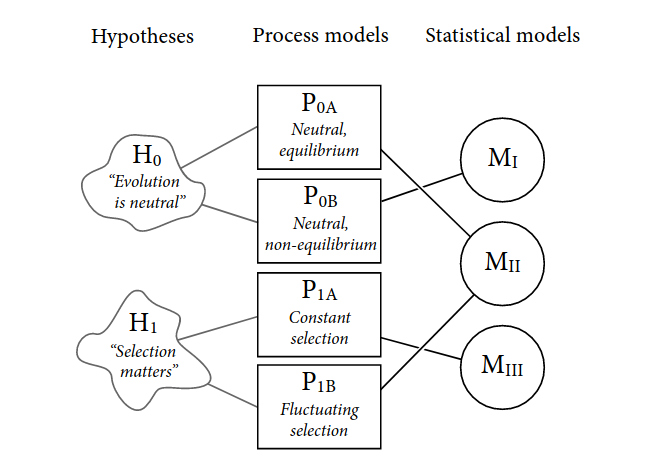
\includegraphics{/home/michael/prospectus/figures/mcelreath.png}
    \caption{From \citet{mcelreath_statistical_2020}--the relationship between hypotheses,
process models, and statistical models represented as a network.
Original caption: \emph{Relations among hypotheses
(/home/michael/prospectus/figures/mcelreath.png), detailed process
models (middle), and statistical models (right), illustrated by the
example of ``neu- tral'' models of evolution. Hypotheses (H) are
typically vague, and so cor- respond to more than one process model (P).
Statistical evaluations of hy- potheses rarely address process models
directly. Instead, they rely upon statistical models (M), all of which
reflect only some aspects of the process models. As a result, relations
are multiple in both directions: Hypotheses do not imply unique models,
and models do not imply unique hypotheses. This fact greatly complicates
statistical inference.}}
\end{figure}

Purely statistical models are certainly not without value. However, for
the purposes of inference and forecasting in biodiversity science, and
complex systems in general, the increasing availability of computing
power to simulate complex process models at large scales have enabled
the gap between process models and statistical models to shrink in
recent years. Methods for fitting empirical data to complex simulation
models has seen much interest in the literature of a wide-variety of
fields in recent years. In the network science and complex systems
literature, methods of this type are typically called ``Bayesian
nonparametrics'' \citep{orbanz_bayesian_2015}), or sometimes ``likelihood-free
inference''. In ecology and evolutionary biology, these methods are
often called Approximate Bayesian Compution (ABC), based on the early
adoption of that nomenclature by Beaumont \citep{beaumont_approximate_2019}), who
used first applied ABC methods in evolutionary genetics in the early 2000s.

In order to understand why ABC has significant potential in ecology, it
is best to start by asking: what is it that makes applying statistical
models to data so much easier than process models? The problem begins
with the difficulty of estimating the value of parameters in a process
model from real data. All models \(f\) have parameters \(\theta\) which
lie outside of what is observable about the model's concepts \(A\). As
an example, consider fitting a species-distribution model (SDM),
\(y = f(x, \theta)\), where \(x\) is the value of an environmental
variable that has been measured across space, and \(y\) is the predicted
probability of a given species being present. To fit this model
\(y =f(x, \theta)\), we need some observed instances of both
environmental conditions \(\hat{x}\) and species occupancy \(\hat{y}\)
in order to estimate \(\theta\)---an ``inverse problem'' whereby we want
to solve the model backwards, so to speak, in order to estimate the
inputs \(\theta\) that produced \(\hat{y}\) given \(\hat{x}\)
\citep{stouffer_all_2019}).

For most statistical data models, there are seemingly endless methods of
estimating \(\theta\) in both frequentist and Bayesian worlds, yet what
the vast majority of these methods have in common is that they estimate
\(\theta\) by using a likelihood function, \(\mathbb{L}({x} | \theta)\),
which is defined as the probability of observing some data point
\(\hat{x}\) given a model definition \(f\) and some parameter values
\(\theta\). In a frequentist world, the likelihood function is a
ubiquitous tool for parameter inference. Most off-the-shelf statistical
`tests', e.g.~ANOVA, are simply a packaged likelihood function that can
be used to quickly estimate parameters for a wide variety of problems
with conceptual similarities. Similarly, in a Bayesian world, the
likelihood function is essential in the application of Bayes' theorem to
inference,

\[ P(\theta | \hat{x}) = \frac{P(\hat{x} | \theta)  P(\theta)}{P(\hat{x})} = \frac{\mathbb{L}(\hat{x}, \theta)  P(\theta)}{\int_\Theta \mathbb{L}(\hat{x} | \theta) P(\theta) d\theta}\]

If our model \(f\) is simple, we can write our likelihood down
analytically, e.g.~if we describe a naive SDM where the probability of
occurrence at a location in space \(L\) is given by the difference
between the ``mean'' trait value of a species, \(T\), and some
environmental condition \(E({L})\) related to the trait in
question\footnote{Of course, capturing the capacity for a species to
  persist using a single dimension is, to say the least, unlikely. The
  oversimplification here is in service of defining the most simple
  model possible.}, we can define a model \(f\) that says the
probability of occurrence at \({L}\) is a Gaussian evaluated at
\(E({L}) - T\), which induces a single parameter,
\(\theta = \{ \sigma \}\). Because our model is defined with an
analytically tractable distribution, we can write down our likelihood
\(\mathbb{L}(x | \theta)\) fairly easily:
\[\mathbb{L}(\text{Species present at} \ {L} \ |\  \sigma) = \frac{1}{\sigma \sqrt{2\pi}} \exp \Big( \frac{-(T-E({L}))^2}{2\sigma^2} \Big)\]

The ability to write our likelihood down in simple analytic termcan be compared to actual datas means
that value of \(\mathbb{L}\) is straightforward to compute for any
values of \(T, E(\vec{L}),\) or \(\sigma\), which is necessary for the
majority of parameter inference methods. Once we estimate \(\sigma\), we
can estimate the probability of occurrence at any point in space \(L\)
by simply evaluating
\(\mathbb{L}(\text{Species present} | E(L) , T, \sigma)\) at that
location, at which point we have a fully-fledged SDM.

What then, if we want to describe a model \(f\) where the probability of
occurrence is driven by both neutral changes in the spatial
distributions of each species, environmental stochasticity, variability
in species' traits in space and time, and so forth? A likelihood
function for this type of process quickly becomes intractable. However,
modern computational power enables us to simulate many replicates of
stochastic simulation models, we can treat the distribution of
simulation model outcomes as approaching the likelihood function as the
number of replicates increases\footnote{There are several caveats here,
  all outside the scope of this document}. One can then use ABC methods
(most of which rely on typical MCMC rejection-sampling) to infer model
parameters, and to use model selection criteria to determine which
mechanistic process, written as a simulation, is more likely to have
produced a set of data.

The contemporary literature surrounding ABC focuses on model validation,
prior selection \citep{jacobs_unified_2014}), methods for sampling
parameters better \citep{beaumont_adaptive_2009}), estimating the
likelihood via regression on simulation data to minimize replicates
\citep{beaumont_approximate_2019})

\begin{itemize}
\item
  \emph{Bayesian \{Models\} of \{Graphs\}, \{Arrays\} and \{Other\}
  \{Exchangeable\} \{Random\} \{Structures\}\}}
  \citep{orbanz_bayesian_2015}
\item
  \emph{Handbook of ABC} \citep{sisson_handbook_2018}
\end{itemize}


% ________________________________________________________________________
%       section 2.2
%           the structure of ecological networks
% ________________________________________________________________________
\hypertarget{the-structure-of-ecological-networks}{%
\subsection{The Structure of Ecological
Networks}\label{the-structure-of-ecological-networks}}

The search for generality among ecological communities long flummoxed
early ecologists, culminating in the aphorism that community ecology is
"a mess" \citep{citation_original}, \citep{vellend_conceptual_2010}).

Early theoretical work on community structure begins with the
Diversity-Stability "Paradox", largely attributed to May \citep{may_will_1972,may_stability_2001}). May found, contrary
to the conventional wisdom at the time, that increasing the diversity of
species in an ecological community decreases its stability. May's work
considered both a linear system, \(\dot{x} = M\vec{x}\), and a
generalized Lotka-Volterra system,
\(\dot{x} = \vec{x} \odot (M \vec{x} + \vec{g})\), where \(\vec{x}\) is
a vector of abundsissonances, \(\vec{g}\) is a vector of change in abundance
absent any consumption and \(M_{ij}\) between any species \(i\) and
\(j\) is the interaction strength\footnote{itself a term fraught with
  ambiguity}. May's generative model of a food web \(M\) with \(N_s\)
species is

\[M = \begin{cases}\sim N(0, \sigma^2) \quad\quad\quad &\text{w.p. }\ c\\ 0 &\text{else}\end{cases}\]

It is important to emphasize that "stable" in this context means
fixed-point stability in a deterministic system. One can compute the
stability of a fixed-point by examining the eigenvalues of the Jacobian
of your system around any fixed point. For both of the models may used,
the Jacobian around a fixed point is always the adjacency matrix, and so
without computing any derivatives we can simply check if the eigenvalues
\(\lambda\) of the adjacency matrix \(M\) all have real component less
than \(0\), i.e.~\(\{ \text{Re}(\lambda) < 0 \} \ \ \forall\lambda\), to
determine if the system has a stable equilibrium. By generating and
evaluating the stability of food-webs this way, May showed as \(N_s\)
increases, the probability that a food web will be stable goes to \(0\).
There is where the so-called `paradox' lies---we observe food-webs in
nature that are woven between far more species than we would expect
under May's model, and so naturally the study of complexity in food webs
turned to both understanding the processes that structure food webs such
that they can persist.

One of the most powerful tools for problem-solving is paying attention
to what is \emph{invariant} about a system, meaning that which does not
change in the system, even as we adjust its parameters
\citep{@polya_how_2009}). Ecosystems vary in seemingly dimensionless ways.
Yet, we can still find an invariant in ecology---the amount of energy
per unit area on the planet is a measurable value, and insofar as we
have any undisputed ``laws'' in science, one that is fairly commonly
accepted is that energy has to go somewhere. The application of
thermodynamics to trophic communities led to a renaissance in our
understanding of food web structure. We directly had measurable things
we could test against a model's expectation, like allometric scaling
\citep{cohen_food_1977, gravel_trophic_2011, stouffer_robust_2006}) and metabolic energy-efficiency in
trophic interactions \citep{yodzis_body_1992}). This enabled us to
develop more sophisticated models of both community structure, in the
form of generative network models \citep{cohen_food_1977,williams_simple_2000} that can be fit to empirical food webs \citep{allesina_general_2008}, and the development of community
dynamics models that are better rooted in thermodynamic constraints. Such models are rooted in MacArthur's Consumer-Resource model \cite{macarthur_cr}, with additional parameters added for metabolic efficiency and energy-use based on allometry \citep{yodzis_body_1992}. These models have much a much stronger empirical basis than LV-type models, but come with the trade-off of, in most cases, analytic intractability. Both these generative models of network structure and dynamics models have been used to study the stability of complex food webs \cite{allesina_stability_2012,allesina_predicting_2015}, and consider more dimensions of stability than May's fixed-point method \cite{dominguezpaper}, and an existing software library \texttt{BioEnergetic.jl} contains a set of generative network models, and a deterministic thermodynamic community model solver \citep{delmas_simulation_2017}.

In parallel, network science has developed
its own set of generative models for network structure which have
several natural applications in food web ecology.
One common feature of empirical ecological networks is they exhibit modularity and nestedness. Understanding the modular structure of networks \footnote{Confusingly, network scientists call this "community structure", but to avoid confusion with ecological communities, we'll avoid this word.} has been a consistent theme in the networks literature for many years \citep{newman, clauset}.
Stochastic-Block-Models (SBMs) have seen extensive use for modular and
nested network structures outside of ecology. Although SBMs are good at detecting modularity and nestedness, there is a trade off between good-fit and information about the process generating the network structure. SBMs only detect patterns in data, they can not on their own tell us how communities are assembled.


% ________________________________________________________________________
%       section 2.3
%           spatial ecology
% ________________________________________________________________________
\hypertarget{spatial-ecology}{%
\subsection{Spatial Ecology}\label{spatial-ecology}}

Spatial ecology as it exists today would be radically different if not
for the Theory of Island Biogeography (TIBG)
\citep{macarthur_theory_2016}. TIBG is a foundation for both
modern spatial and community ecology, and further provides a mechanistic
explanation for the species-area relationship, one of the most
well-established "laws" in ecology. The conceptual construction of
space used by TIBG---a set of internally homogeneous `islands', each
variable in size and surrounded by inhospitable water/matrix, each
either occupied or unoccupied by a particular species and connected via
dispersal---had deep impacts on the methodology and models used to study
ecological patterns across space. Around the same time, metapopulation
theory, coined by Levins \citep{levins_demographic_1969}, more
explicitly explored occupancy dynamics. Much like TIBG, Levins
considered as system of isolated patches, each either occupied or
unoccupied in time. The proportion of patches \(p\) occupied at any time
was modeled as

\[\frac{dp}{dt} = pc(1-p) - cp\]

where \(c\) is the instantaneous probability of colonization and \(e\)
is the instantaneous probability of extinction of any given patch. From
this Levins derived that the system will only persist if
\(\frac{c}{e} > 1\). Levins' Metapopulation model and TIBG share much in
common, all patches are homogeneous in that they all are colonized or go
extinct with the same probability as every other patch, and it is
assumed that each system progresses toward an equilibrium state over
time. The assumption of uniform colonization and extinction rates across
all patches was eventually challenged by Hanski and Ovaskainen, who
developed a spatially-explicit model of metapopulation dynamics
\citep{hanski_practical_1994}) , where a finite number of populations each has
an explicit location in space, an area (which is a proxy for resource
availability, much like TIBG), and a unique probability of colonization
of extinction based both on the physical proximity to other patches and
the occupancy state of the rest of the system. Further, the increased
availability of computer power in the 1990s enabled the first simulation
models to be applied in spatial ecology. Many studies focused on the
effects of habitat structure and loss by simulating occupancy dynamics
on a lattice and measuring the probability of metapopulation persistence
\citep{bascompte_habitat_1996}, etc) .

Although TIBG and both Levins' and Hanski's metapopulation models rely
on discrete-space constructions of space, a tension counter to discrete
space runs throughout modern spatial ecology. The increasing
availability of remote-sensing data has enabled the first `continuous'
ecological data. As satellites designed for Earth Science orbit the
Earth, they bounce electromagnetic signals off the surface of our
planet, and record the spectral signature they receive reflected back at
them. The reflective signature of Earth's terrain can then be used to
estimate various properties about its surface---land cover, hydrology
and topography, abundance of abiotic resources like nitrogen and
phosphorus, and so on. The properties used by both different satellites
and different models vary widely in what they try to predict---from the
level of coarse land-cover categorizations to the presence of particular
species \citep{cite}. Further, there is considerable variability in the spatial and
temporal scale at which data is collected--however, it is still hard to
overstate the potential value of large-scale raster data in ecological
forecasting, as we now have methods to build complex models of habitat
suitability and dispersal using resistance surfaces \citep{cite}),
which have the potential to integrate nicely with climate and land-use
forecasting models derived from other fields (\cite{dietze}).




% ________________________________________________________________________
%       section 2.4
%           metacommunities
% ________________________________________________________________________
\hypertarget{metacommunities}{%
\subsection{Metacommunities}\label{metacommunities}}

Leibold et al.~\citep{leibold_metacommunity_2004} introduced
the metacommunity framework a synthesis of community and spatial
ecology. They define four paradigms under which previous research on the
interplay of community and spatial ecology can be categorized: 1) the
Species-Sorting perspective, 2) the Patch-Dynamics perspective, 3) the
Mass-Effect Perspective, and 4) the Neutral perspective.

Although understanding the effects of spatial processes on community
structure has been a crucial part of the discipline since its rapid
growth in the 1950s and 1960s \citep{hutchinson_ecological_1973},
\citep{chase_ecological_2003}), this work only considered space solely as a
domain across the environment varies--- each species was considered a
static object in space in time, which are distributed according to
selection on environmental variables. This forms the theoretical basis
for niche theory \citep{hutchinson_ecological_1973,chase_ecological_2003}, as a mechanism behind community assembly, or what
Leibold et al.~call the Species-Sorting perspective of metacommunity
dynamics. The Patch-Dynamics perspective is rooted in the TIBG from
above--occupancy dynamics on discrete, internally homogeneous
patches/islands, where diversity is limited by dispersal and not
resource availability. The Mass-Effect perspective shifts to systems
where dispersal drives patterns of local demography, rather than
occupancy dynamics---sources and sinks (pulham, etc.). Finally, the
Neutral perspective considers community dynamics driven by random drift,
i.e.~dynamics at scales where there is not enough variability in either
selection or dispersal to drive variation of community structure across
space, beyond than the variability attributable to the inherent
stochasticity of population dynamics.

The methods used in each of the domains of these paradigms often
differed drastically---however Velland 2010 \citep{vellend_conceptual_2010} argues
that within each of these four perspectives we see the same four
fundamental processes driving dynamics, just in different amounts.
Velland's four processes are Selection, Dispersal, Drift, and
Speciation--functionally the same as the four fundamental processes in
evolutionary genetics, which similarly deals with shifting compositions
of units of over space and time, the difference being that evolutionary
genetics deals with alleles, not species. These fundamental processes
have been used in recent years to develop \emph{process-based} models of
metacommunity dynamics, which aim to provide a mechanistic explanation of metacommunity structure
\citep{poisot_2014}, \citep{thompson}).

Several questions remain---at what different levels of each of the four
processes do communities move between Leibold et al.'s four
prespectives?



% ________________________________________________________________________
%
%       CHAPTER 3
%
%           a metacommunity model
%
% ________________________________________________________________________

\hypertarget{a-metacommunity-model}{%
\section{A Metacommunity Model}\label{a-metacommunity-model}}

Here we describe a process-based simulation model of metacommunity
dynamics across space, which will be implemented as a software toolkit
which will be used for each research chapter in the dissertation.


% ________________________________________________________________________
%       section 3.1
%           what can we measure
% ________________________________________________________________________
\hypertarget{what-can-we-measure}{%
\subsection{What can we measure?}\label{what-can-we-measure}}

In the last section we explored how it is essential for a model \(f\) to
interface with observable quantities \(O(A)\) of the conceptual objects
\(A\) that \(f\) is built with. Much of what drives community dynamics
in space and time is not directly observable to us--the evolutionary
life histories of organisms lie outside the temporal limits of our
observation, as do the ecological conditions of the more-than extremely
recent past, only what we can infer. What we can directly
observe--abundance/occupancy at a given time, traits or genomes sampled
from individuals, etc.--are subject to the limitations of exhaustive
field work, which can only be done on relatively small spatial scales.
We have databases composed of occupancy/abundance data, traits, inferred
phylogenetic history, and interactions (mangal paper, ncbi, etc), but
there is often much variability in the resolution of this data. For
abiotic variables, we can collect, with variable but ever-improving
spatial and temporal resolution, environmental variables like
temperature, precipitation, as well as land-usage maps, and more
recently, topographical and hydrological models of the Earth's surface.
From other fields we also have well-developed predictive models of
climatology, hydrology, and land-use, which can serve as inputs into our
predictive ecological models.



% ________________________________________________________________________
%       section 3.2
%           a four part metacommunity model
% ________________________________________________________________________
\hypertarget{the-four-parts-of-a-metacommunity-model}{%
\subsection{The Four Parts of a Metacommunity
Model}\label{the-four-parts-of-a-metacommunity-model}}

Here, we divide our metacommunity model into four parts:

\begin{enumerate}
\def\labelenumi{\arabic{enumi}.}
\item
  \textbf{Metaweb Model}: \(\{M, B, \frac{\partial B}{\partial t}\}\)

  The Metaweb model consists of the topology of the metaweb \(M\), and
  the way the biomass \(B\) flows through the metaweb,
  \(\frac{\partial B}{\partial t}\). The metaweb \(M\) can be derived
  empirically, or built from a generative model
  \citep{williams_martinez}, \citep{allesina}).
  \(\frac{\partial B}{\partial t}\) can be a deterministic model (like
  used in \citep{delmas}, thompson, dakos stability), or include
  stochasticity and trait-matching as part of the functional response.
\item
  \textbf{Spatial Model}: \(\{L, S, H, E, \Phi \}\)

  We have some set of locations \(L\) in a spatial domain \(S\). This
  representation of landscape structure maps onto the most common
  spatial representations in ecology: patch-based, spatial graph, and
  raster/lattice---see Figure 2. Each location \(L\) is associated with
  a values of environmental variables \(E(L)\) and of habitat
  suitability \(H_i(L)\) for each species \(i\), which is empirically
  derivable from various existing models at either large scales (SDMs)
  or small scales (resistance surfaces/land use) or can be generated
  using any number of methods for generating spatially auto-correlated
  data---see Figure 3. Finally, the spatial model includes a dispersal
  potential \([\Phi^{(i)}_{xy}]\), which is the instantaneous
  probability that a unit of biomass from species \(i\) moves from
  \(x \to y \quad \forall x,y \in S\). The value of \(\Phi^{(i)}_{xy}\)
  is derivable from a resistance surface produced via Curcuitscape
  {[}\citep{cite}{]}, or can be modeled as a function of
  isolation-by-distance using a dispersal kernel \citep{hanski}, who
  knows all of them).

  \begin{figure}[H]
  \centering
  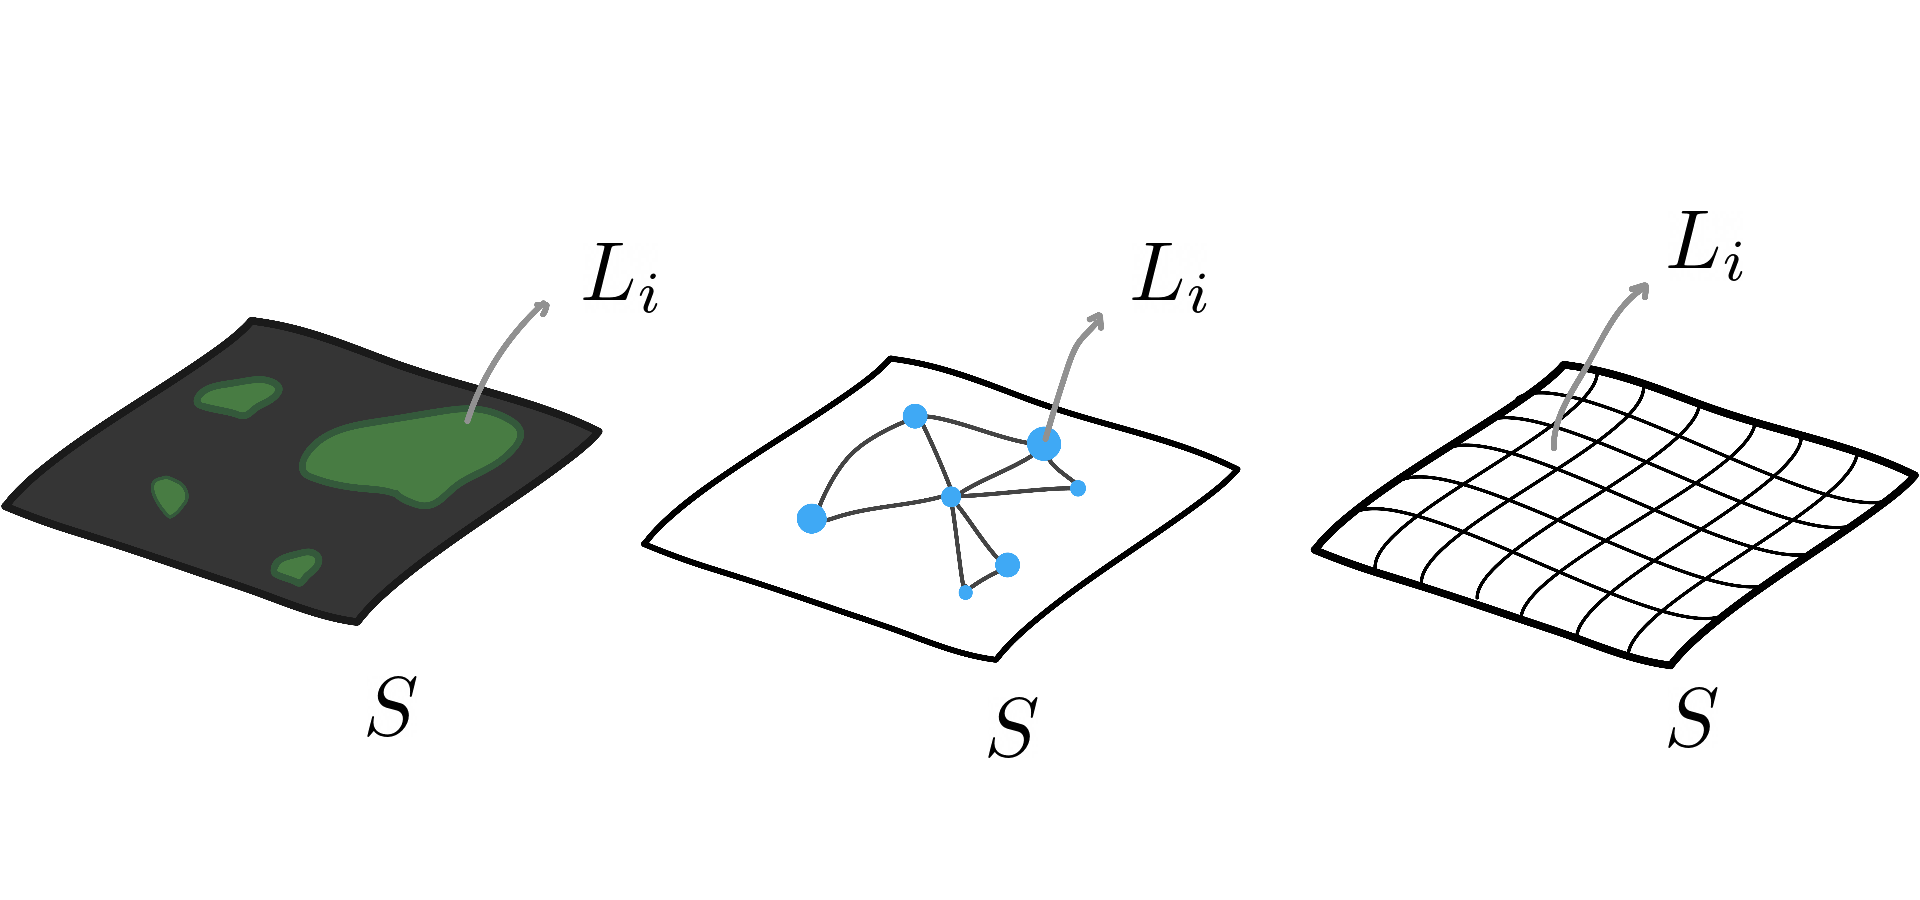
\includegraphics{/home/michael/prospectus/figures/different_spatial_models_w_labels.png}
  \caption{this is a caption}
  \end{figure}

  \begin{figure}[H]
  \centering
  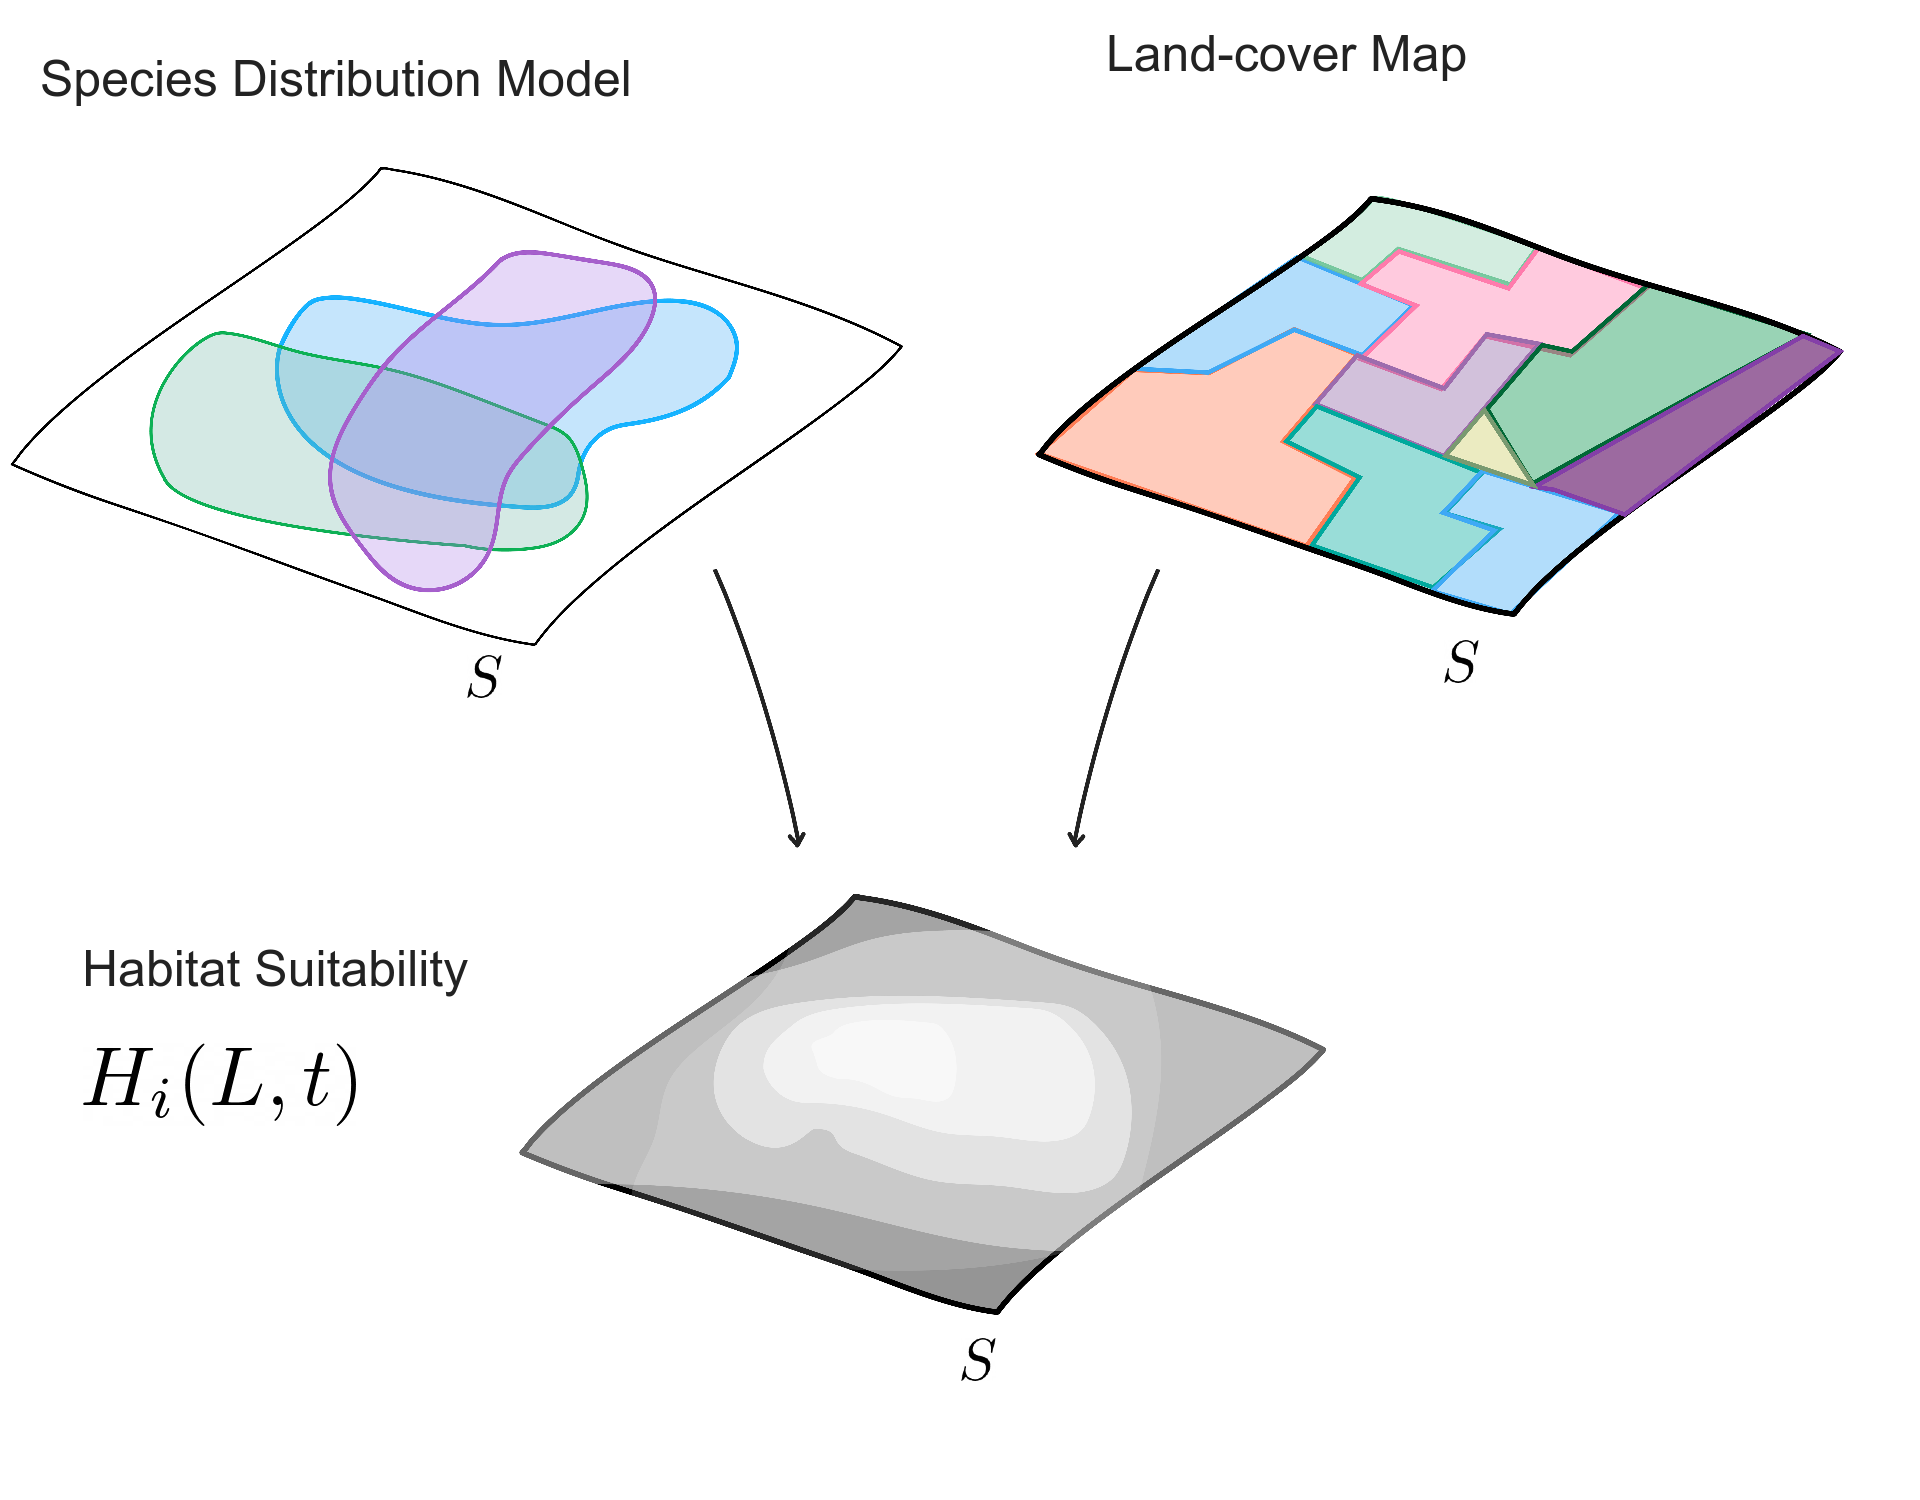
\includegraphics{/home/michael/prospectus/figures/habitat suitability w labels.png}
  \caption{this is a caption}
  \end{figure}
\item
  \textbf{Selection Model}: \(\{ E, T, \frac{\partial T}{\partial t}\}\)

  The selection model describes the traits \(T_i(L)\) of each species
  \(i\) at a location \(L\), and some function
  \(\frac{\partial T}{\partial t}\) which describes how \(T_i(L)\)
  changes over time as a function of both \(E(L)\) and \(T_i(L)\), which
  has several candidates from early evolutionary biology
  \citep{cite}). Further, the selection model could include some
  measure of speciation based on differences in \(T_i\), however it
  doesn't directly relate to the questions in the proposed chapters.
\item
  \textbf{Community Summary Model}: \(\{ C(\hat{B}) \}\)

  Finally, the Community Summary model is a summary statistic which maps
  from the observed state of biomass abundance (or occupancy)
  \(\hat{B}\) at some place and time to a value that representscan be compared to actual data
  community structure, e.g.~Shannon-entropy as a measure of
  \(\alpha\)-diversity. \(C\) could also be a measure of \(\beta\) or
  \(\gamma\)-diversity. If we are using a measure of
  \(\alpha\)-diversity, we may include an additional summary statistic
  to encapsulate the distribution of \(C\) across all locations \(L\).
  See Figure 4. One goal with the metacommunity model is to compare
  various metacommunity summary statistics to explore how they covary.
  Further, if summary statistics are not differentiable even when the
  generative process is different, that itself is interesting, and, in
  general, simulation models are excellent testing grounds for the
  biases of summary stats.
\end{enumerate}

\begin{figure}[H]
\centering
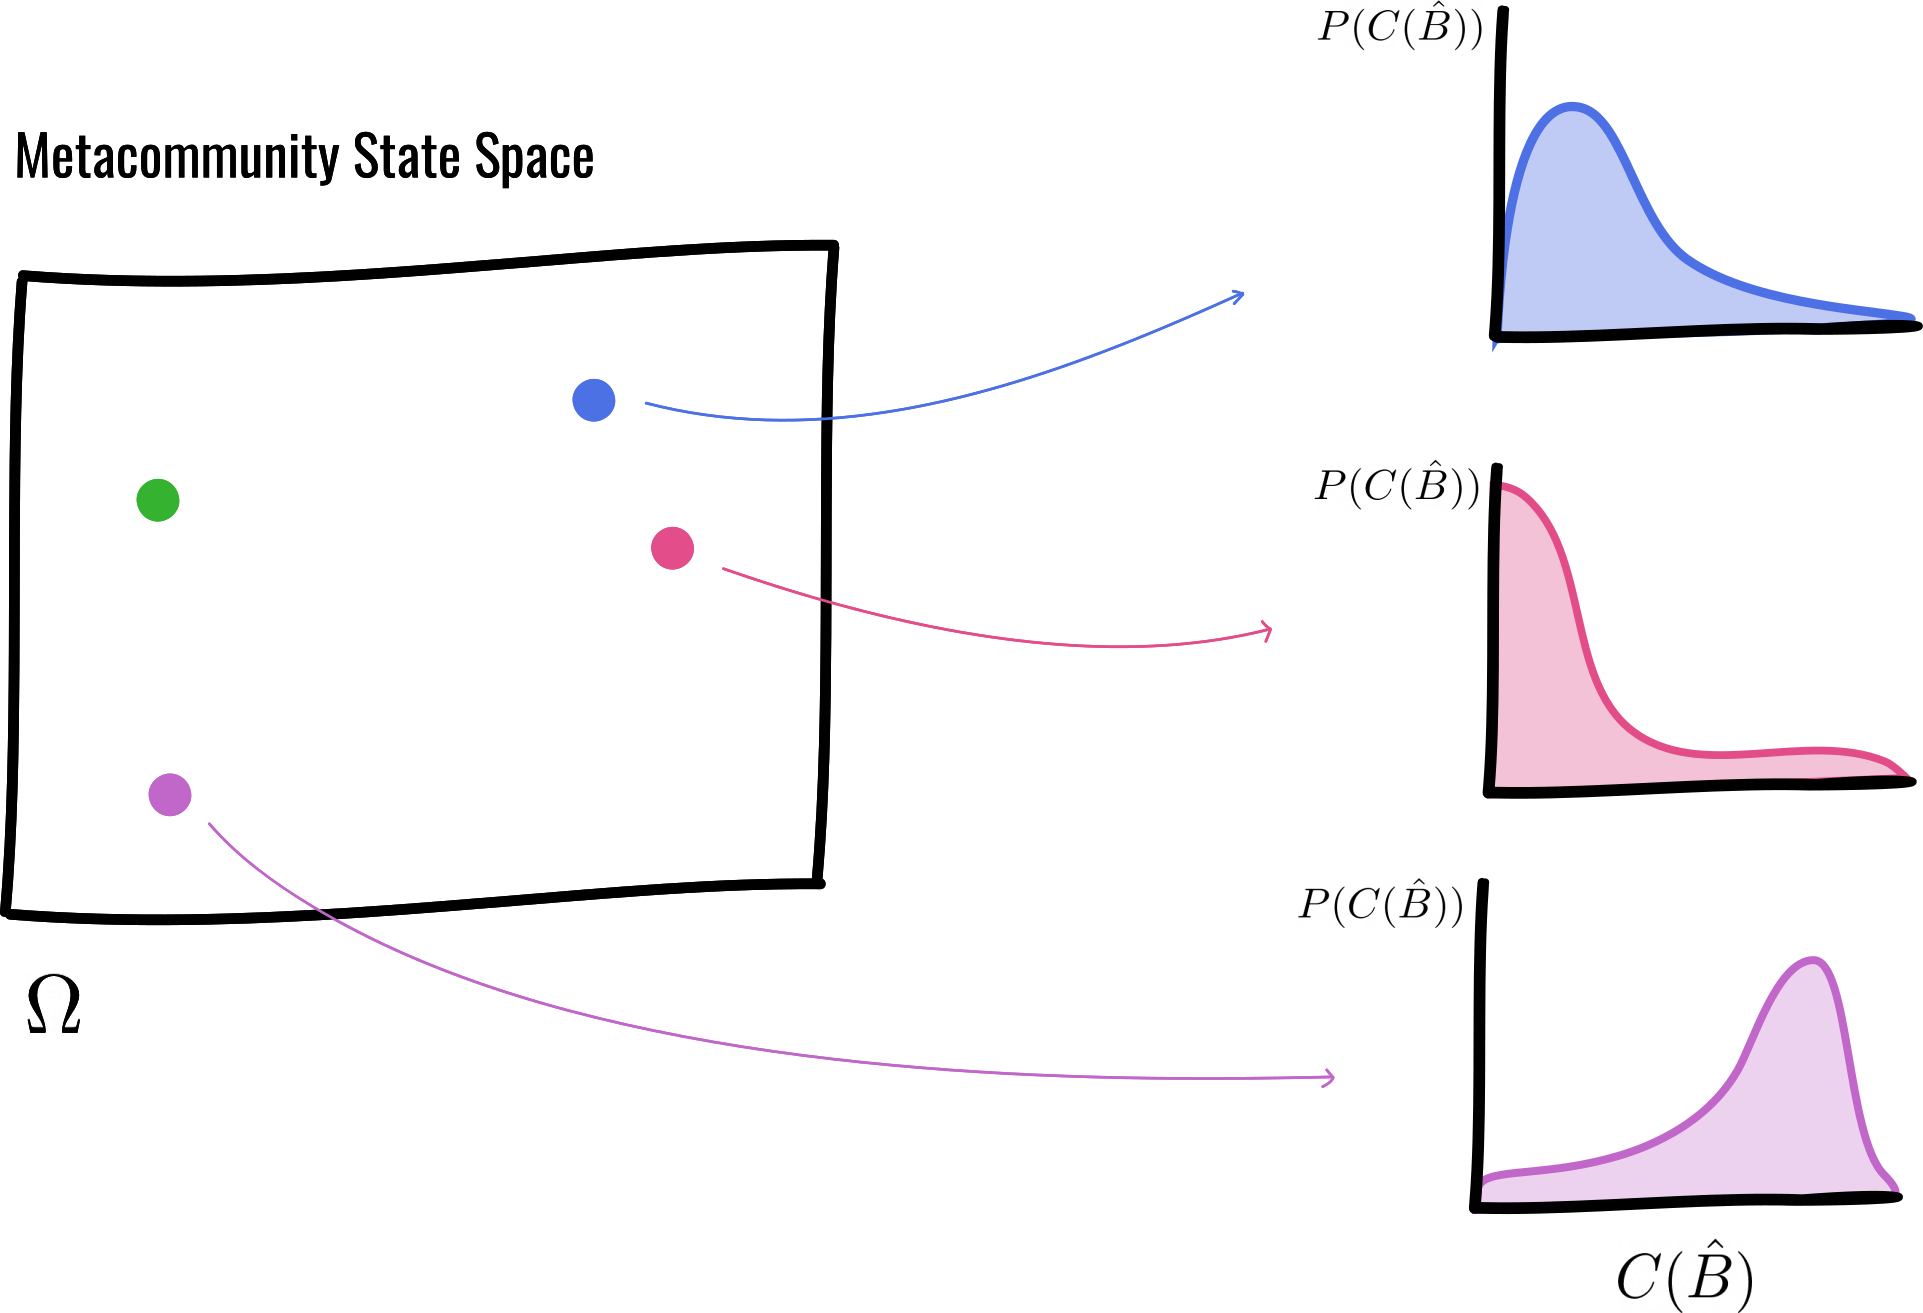
\includegraphics{/home/michael/prospectus/figures/metacomm_w_distributions.png}
\caption{this is a caption}
\end{figure}

% ________________________________________________________________________
%       section 3.3
%           software implementation
% ________________________________________________________________________
\hypertarget{software-implementation}{%
\subsection{Software Implementation}\label{software-implementation}}

Here, we describe how we will implement this metacommunity model as a
modular toolbox of software to simulate metacommunity dynamics that
interfaces with actual data and can be applied forecast in real systems.

\hypertarget{interfacing-with-generative-models-and-data}{%
\subsubsection{Building an Instance of the Model}
\label{interfacing-with-generative-models-and-data}}
In Figure 5 we can see how the conceptual objects in our metacommunity
model
\(A = \{B, L, M, T, \Phi, H, C, \frac{\partial B}{\partial t}, \frac{\partial T}{\partial t} \}\)
can interface with both generative models for the sake of using the
software as a ``virtual laboratory'' \citep{volker_grimm} and
empirical data to forecast in real systems. The point is not necessarily
to vary all elements at once, but instead to have a modular set of tools
that cover a wide variety of use-cases. For example, if for a given use-case, selection is not a relevant part of the question being asked, one could remove selection on traits from the model entirely.

\begin{figure}[H]
\centering
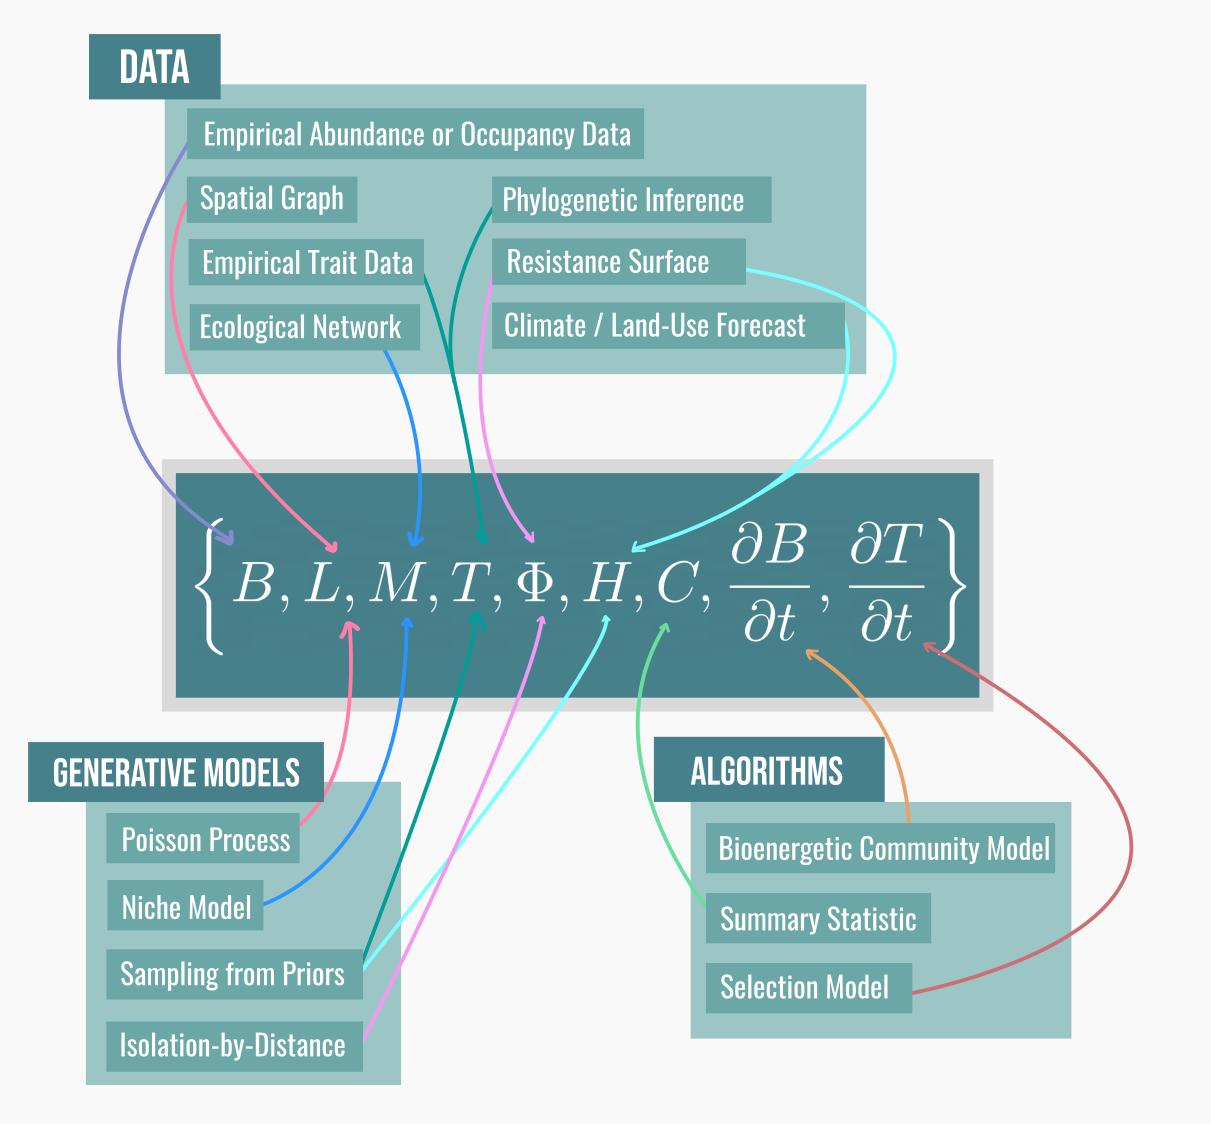
\includegraphics{/home/michael/prospectus/figures/inputs.png}
\caption{this is a caption}
\end{figure}



\hypertarget{finding-the-pseudoequilibria-of-our-metacommunity-model}{%
\subsubsection{Describing Metacommunity Dynamics}
\label{finding-the-pseudoequilibria-of-our-metacommunity-model}}

For any given instance of a model $\hat{A} = \{B, L, M, T, \Phi, H, C, \frac{\partial B}{\partial t}, \frac{\partial T}{\partial t} \}$, one can then simulate the dynamics of the community, at which point we have a sampled trajectory $B(t) \ \ \forall t \in \tau$ where $\tau$ is the simulation time domain. From this, we apply our summary statistic $C(B(t)) \ \ \forall t \in \tau$, and we have a trajectory in summary statistic space $\Omega$---see figure ref. After running our model for many replicates, we can compute a density over the state-space $\Omega$ which represents the proportion of time the model spent in that part of $\Omega$. Do most models tend to converge to a small area of $\Omega$, and sit in pseudoequilibrium?


\begin{figure}[H]
\centering
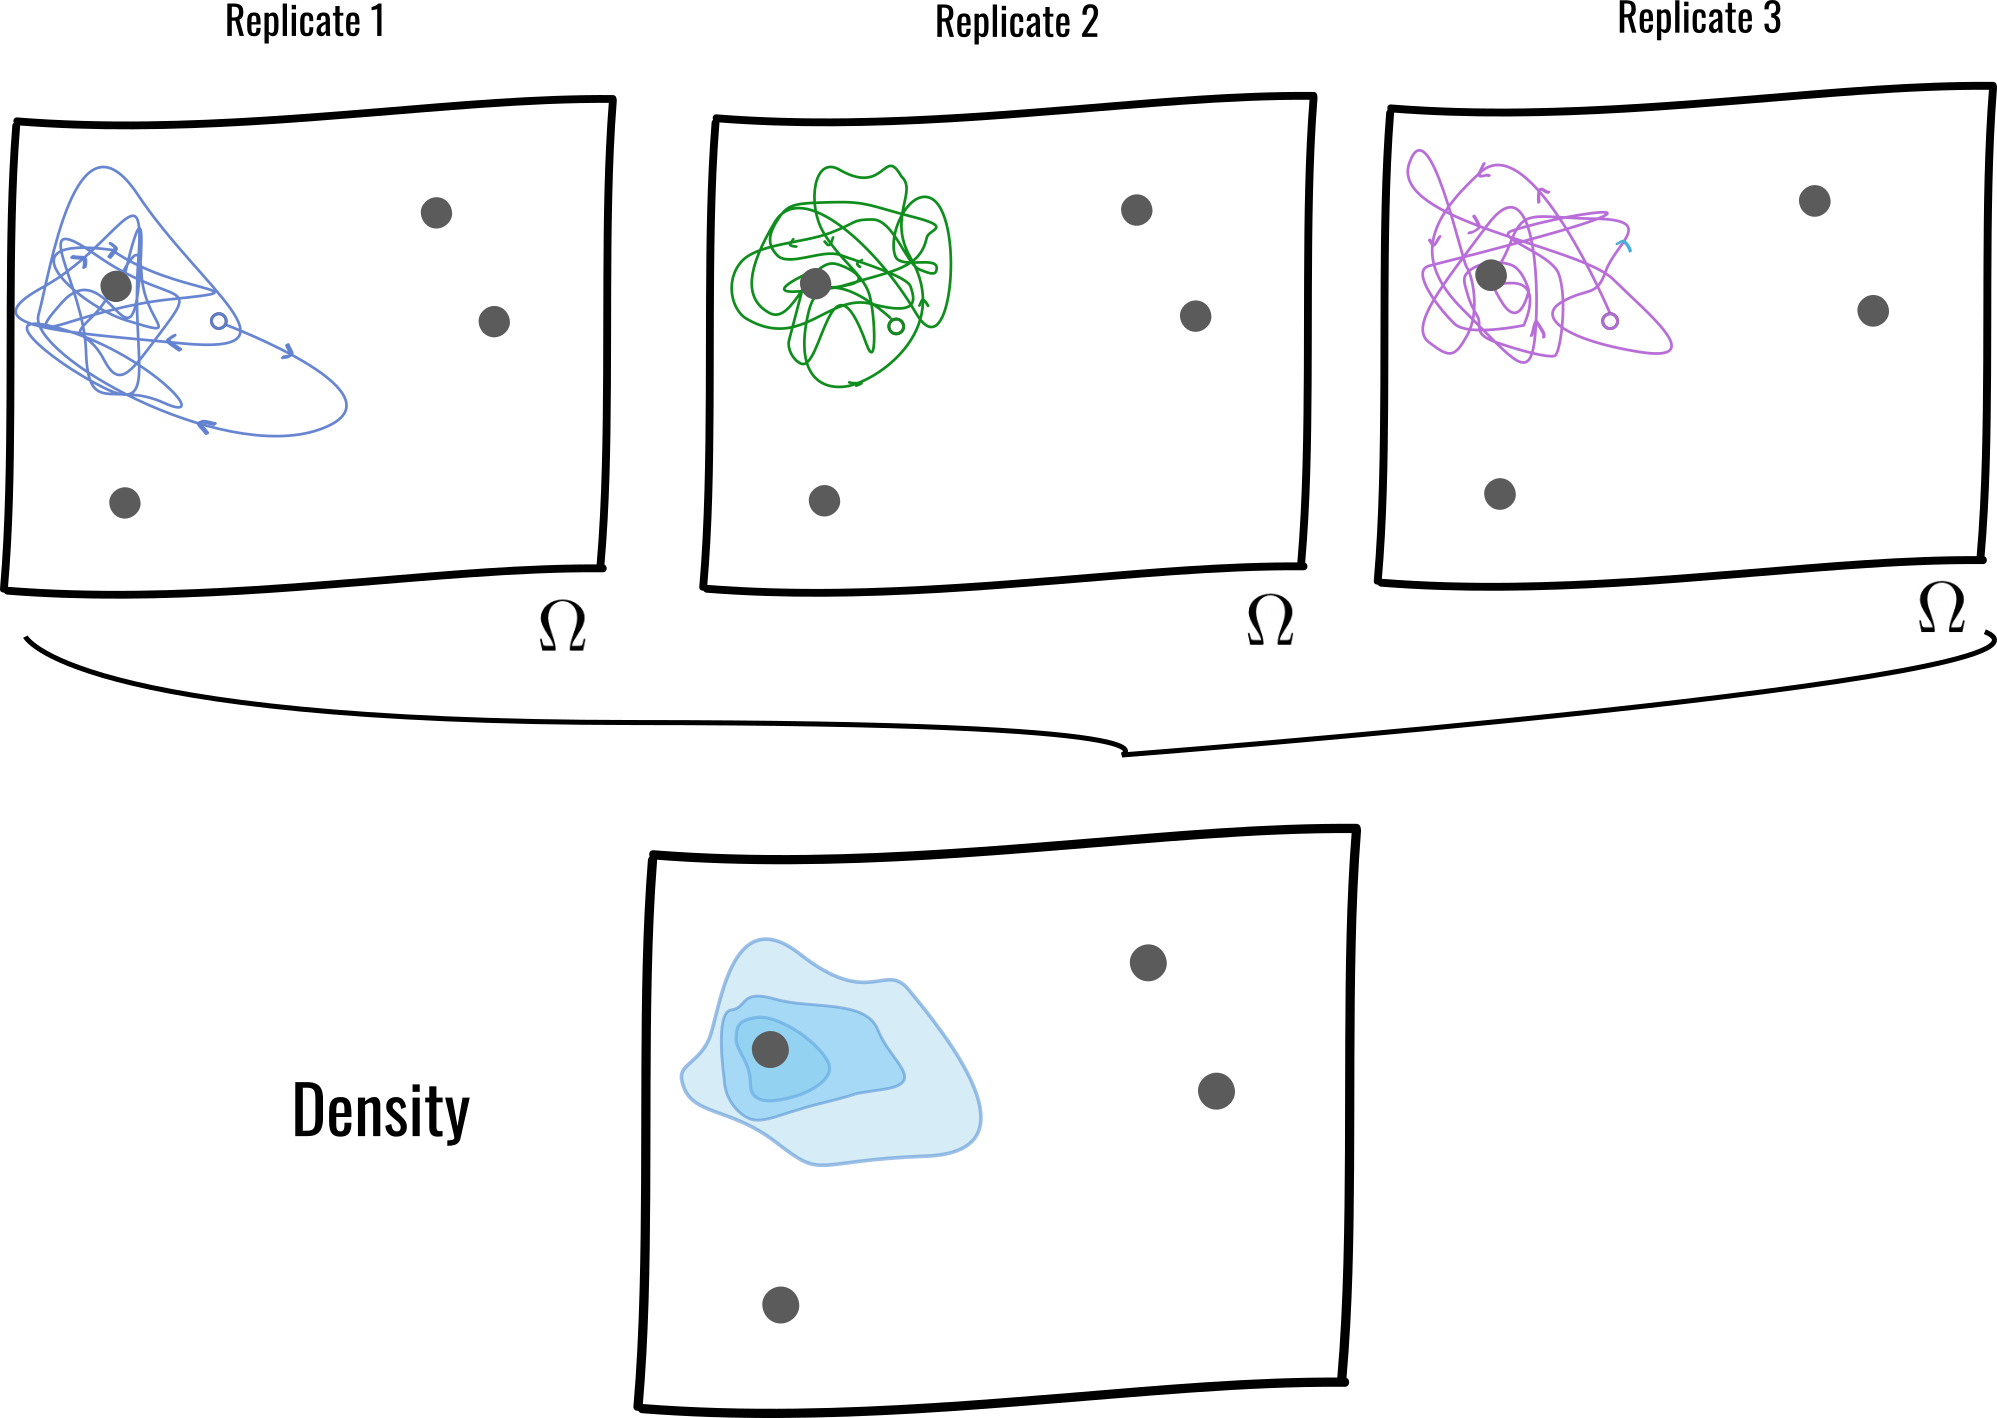
\includegraphics{/home/michael/prospectus/figures/density_plot.png}
\caption{this is a caption}
\end{figure}

\hypertarget{fitting-to-data-with-abc}{%
\subsubsection{Fitting Simulations to Data with
ABC}\label{fitting-to-data-with-abc}}

In order to fit this metacommunity model to real data, we'll build an ABC sampler which takes in a definition of a simulation model $\hat{A}$
and a set of priors with hyperparameters
$\text{Priors}(\chi)$ as inputs, and estimates the posterior distribution---see Figure acb.

The version of an ABC Sampler presented here is methodologically the
simplest (and original) version, based on using a simulated likelihood
to run a rejection-based sampling MCMC algorithm. In the
top-right panel of figure ref, to actually compute \(\mathbb{L}(\hat{y} | \theta)\) from
simulation outputs under \cite{beaumont_adaptive_2003}, one defines an acceptance tolerance
\(\rho\), and accepts $\mathbb{L}(y_{sim} | \theta) = \mathbb{L}(\hat{y} | \theta)$ if \(|\hat{y} - y_{sim}| < \rho\) . Alternatively, one
can run a regression on the on the simulation outcomes to get an
analytic approximation of \(\mathbb{L}(\hat{y} | \theta)\) \cite{whodidthis}. More recent
improvements to ABC sampling deviate from simple rejection sampling
algorithms for efficiency, e.g.~doing rejection sampling whilst
composing the simulated likelihood to reduce the amount of time spent
running the simulation model in ``bad'' regions of parameter space---see
Adaptive Monte Carlo \citep{beaumont_adaptive_2009} and Sequential
Monte Carlo \citep{cite}.

To do this, the sampler draws a set of parameters
 $\hat{\theta} \sim \text{Priors}(\chi)$
and runs the simulation procedure described in the previous section to describe a density in
$\Omega$ that approximates the likelihood function,
$\mathbb{L}(C(B) | \hat{\theta})$, and then uses this approximated likelihood to estimate the posterior distribution
$P(\theta | \hat{y})$.

\begin{figure}[H]
\centering
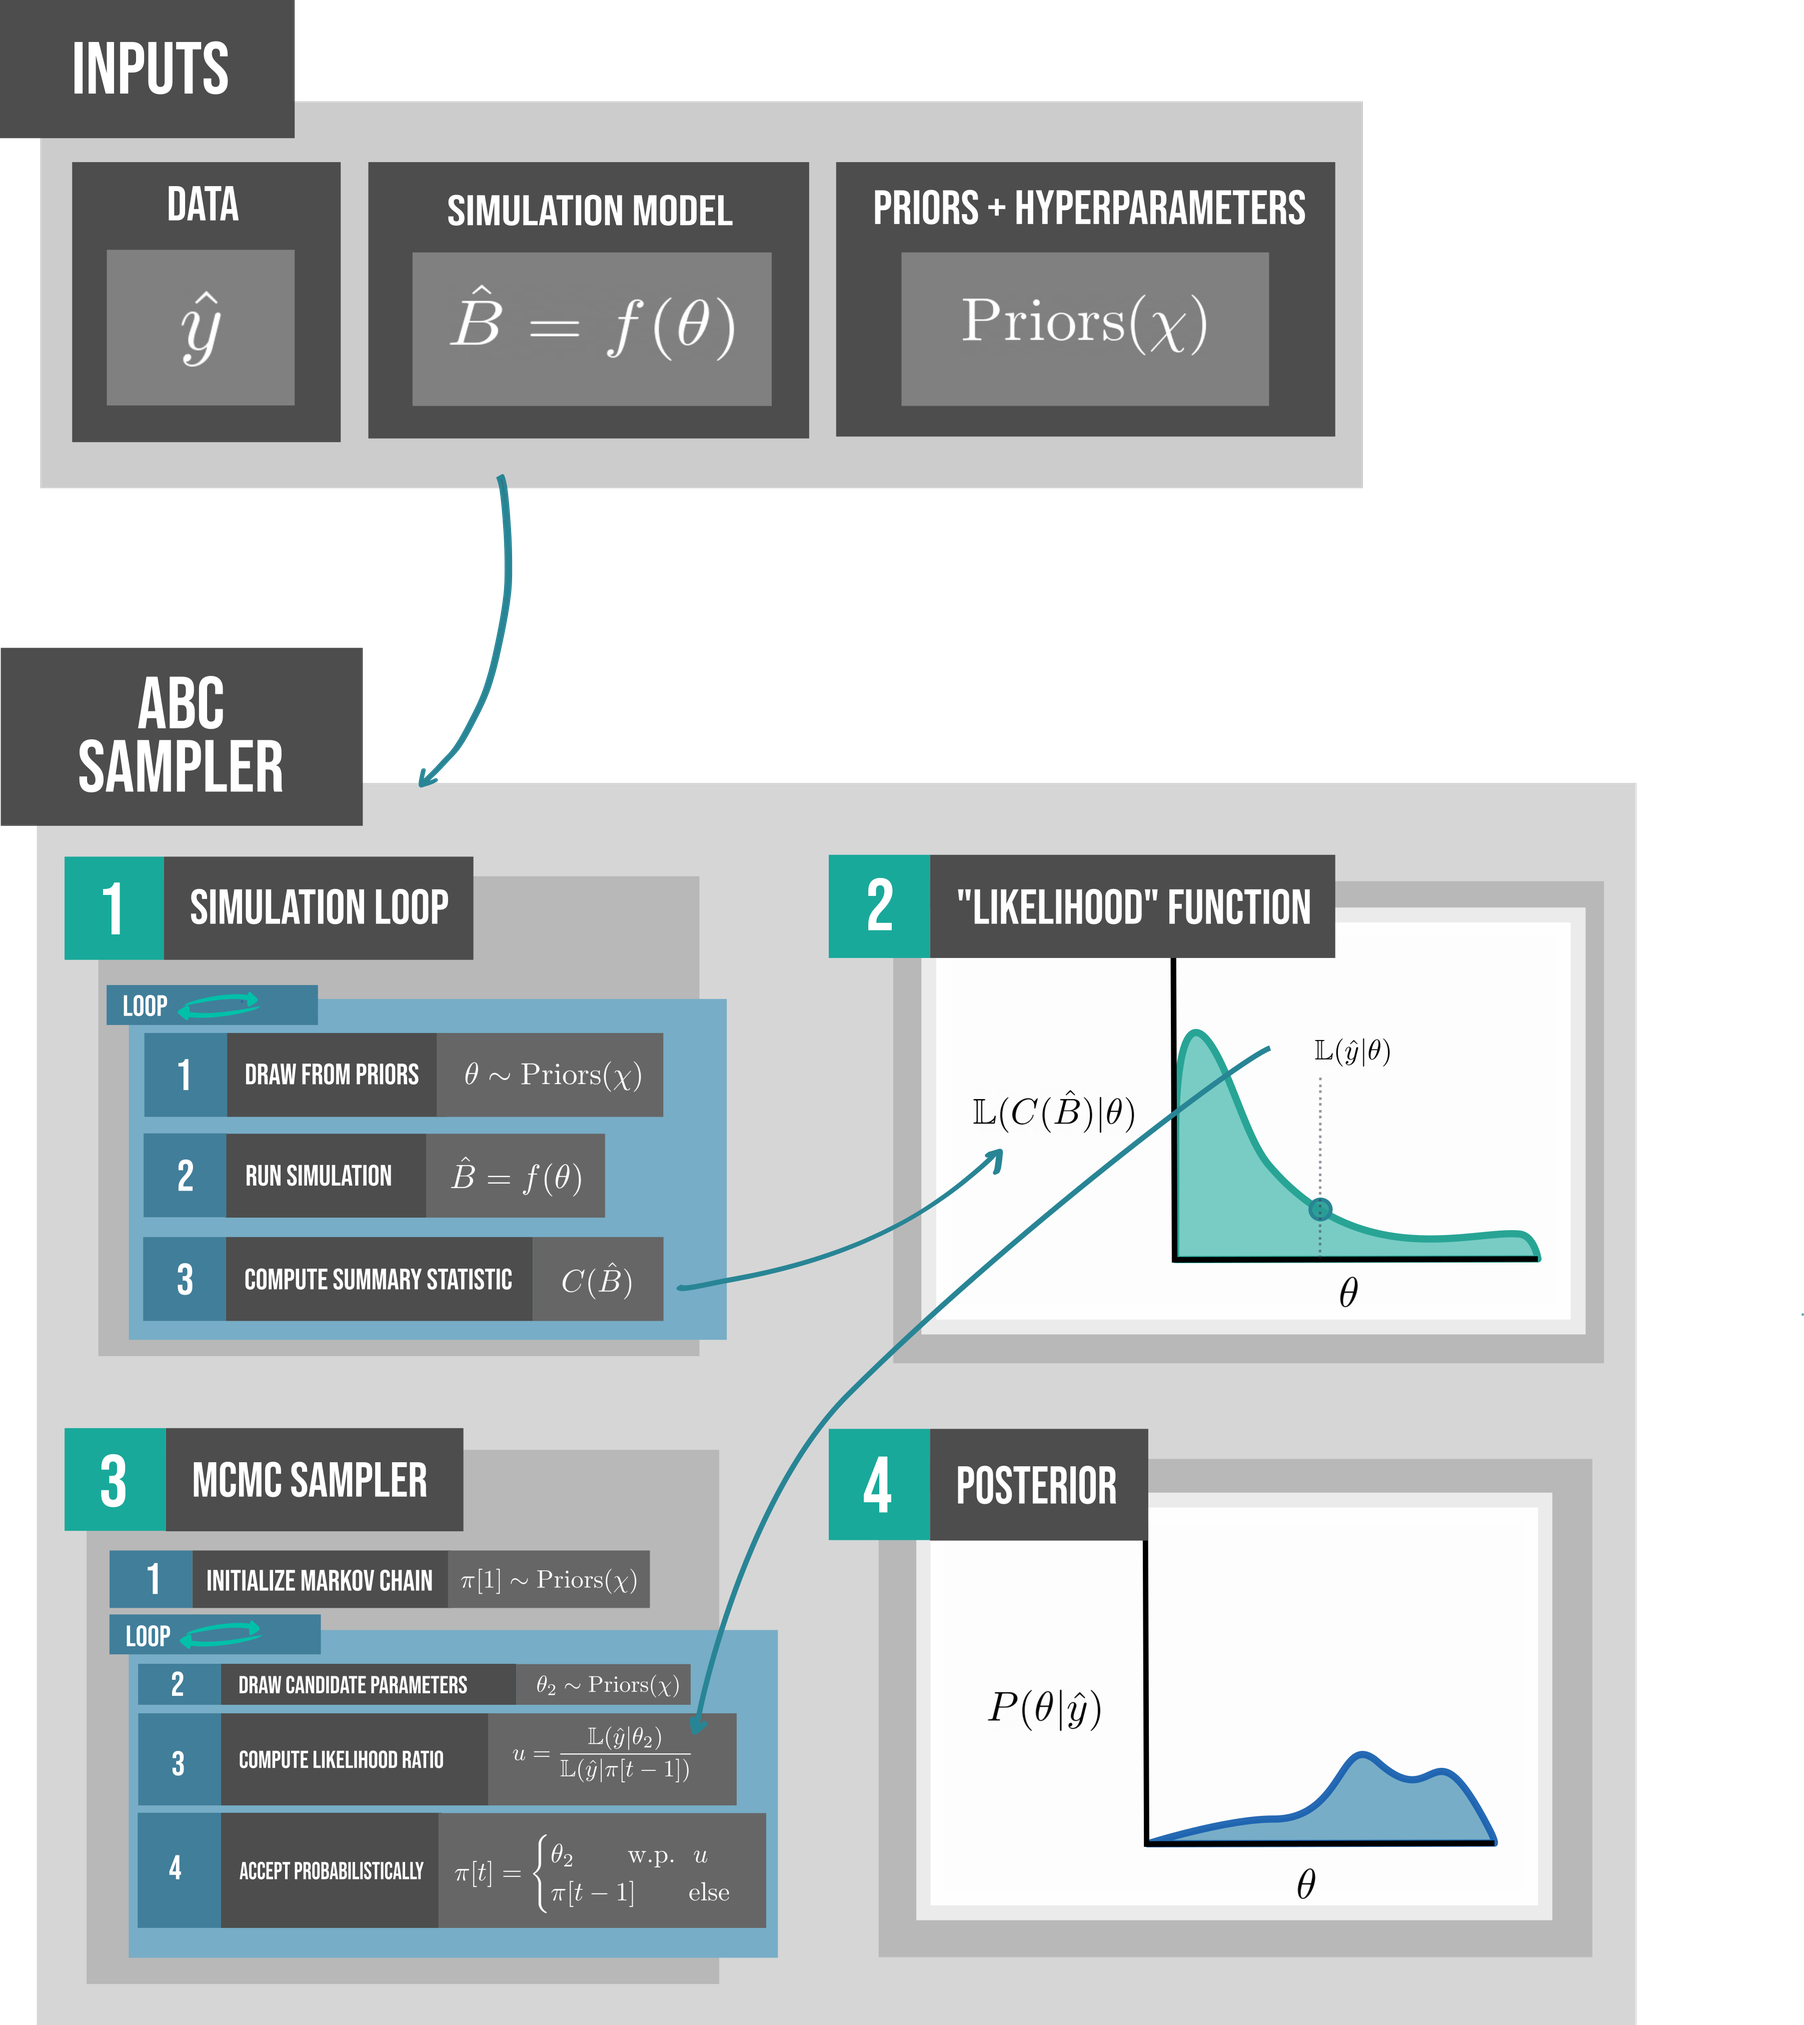
\includegraphics{/home/michael/prospectus/figures/abc_conceputal.png}
\caption{Conceptual overview of an Approximate Bayesian Computation (ABC) Sampler.
}
\end{figure}

If we have several competing simulation models or sets of hyperpriors, we can compare them using information criterion to see which one best describes the data.


\hypertarget{choosing-models-and-priors}{%
\subsubsection{Choosing Models and Priors}\label{choosing-models-and-priors}}

In order to select which version of a simulation model (e.g. deterministic vs. stochastic dispersal) and set of priors gives our model the most predictive power, we need a method for applying an information criterion to a set of models and priors--see figure not done yet.

\hypertarget{forecasting}{%
\subsubsection{Forecasting}\label{forecasting}}

Once we've estimated the best fitting posterior distribution $P(\theta | \hat{y})$, we can use it for forecasting via the best fitting simulation model. We can simply draw $\hat{\theta} \sim P(\theta | \hat{y})$ and run the dynamics model forward. After doing this many times, we get a density of predicted outcomes across the time domain $\tau$. If we have a forecasted model of land-use or climate change, we can also use that as an input into the model to shift $E_i(L, t)$ and $H_i(L,t)$ over time as well.

\begin{figure}[H]
\centering
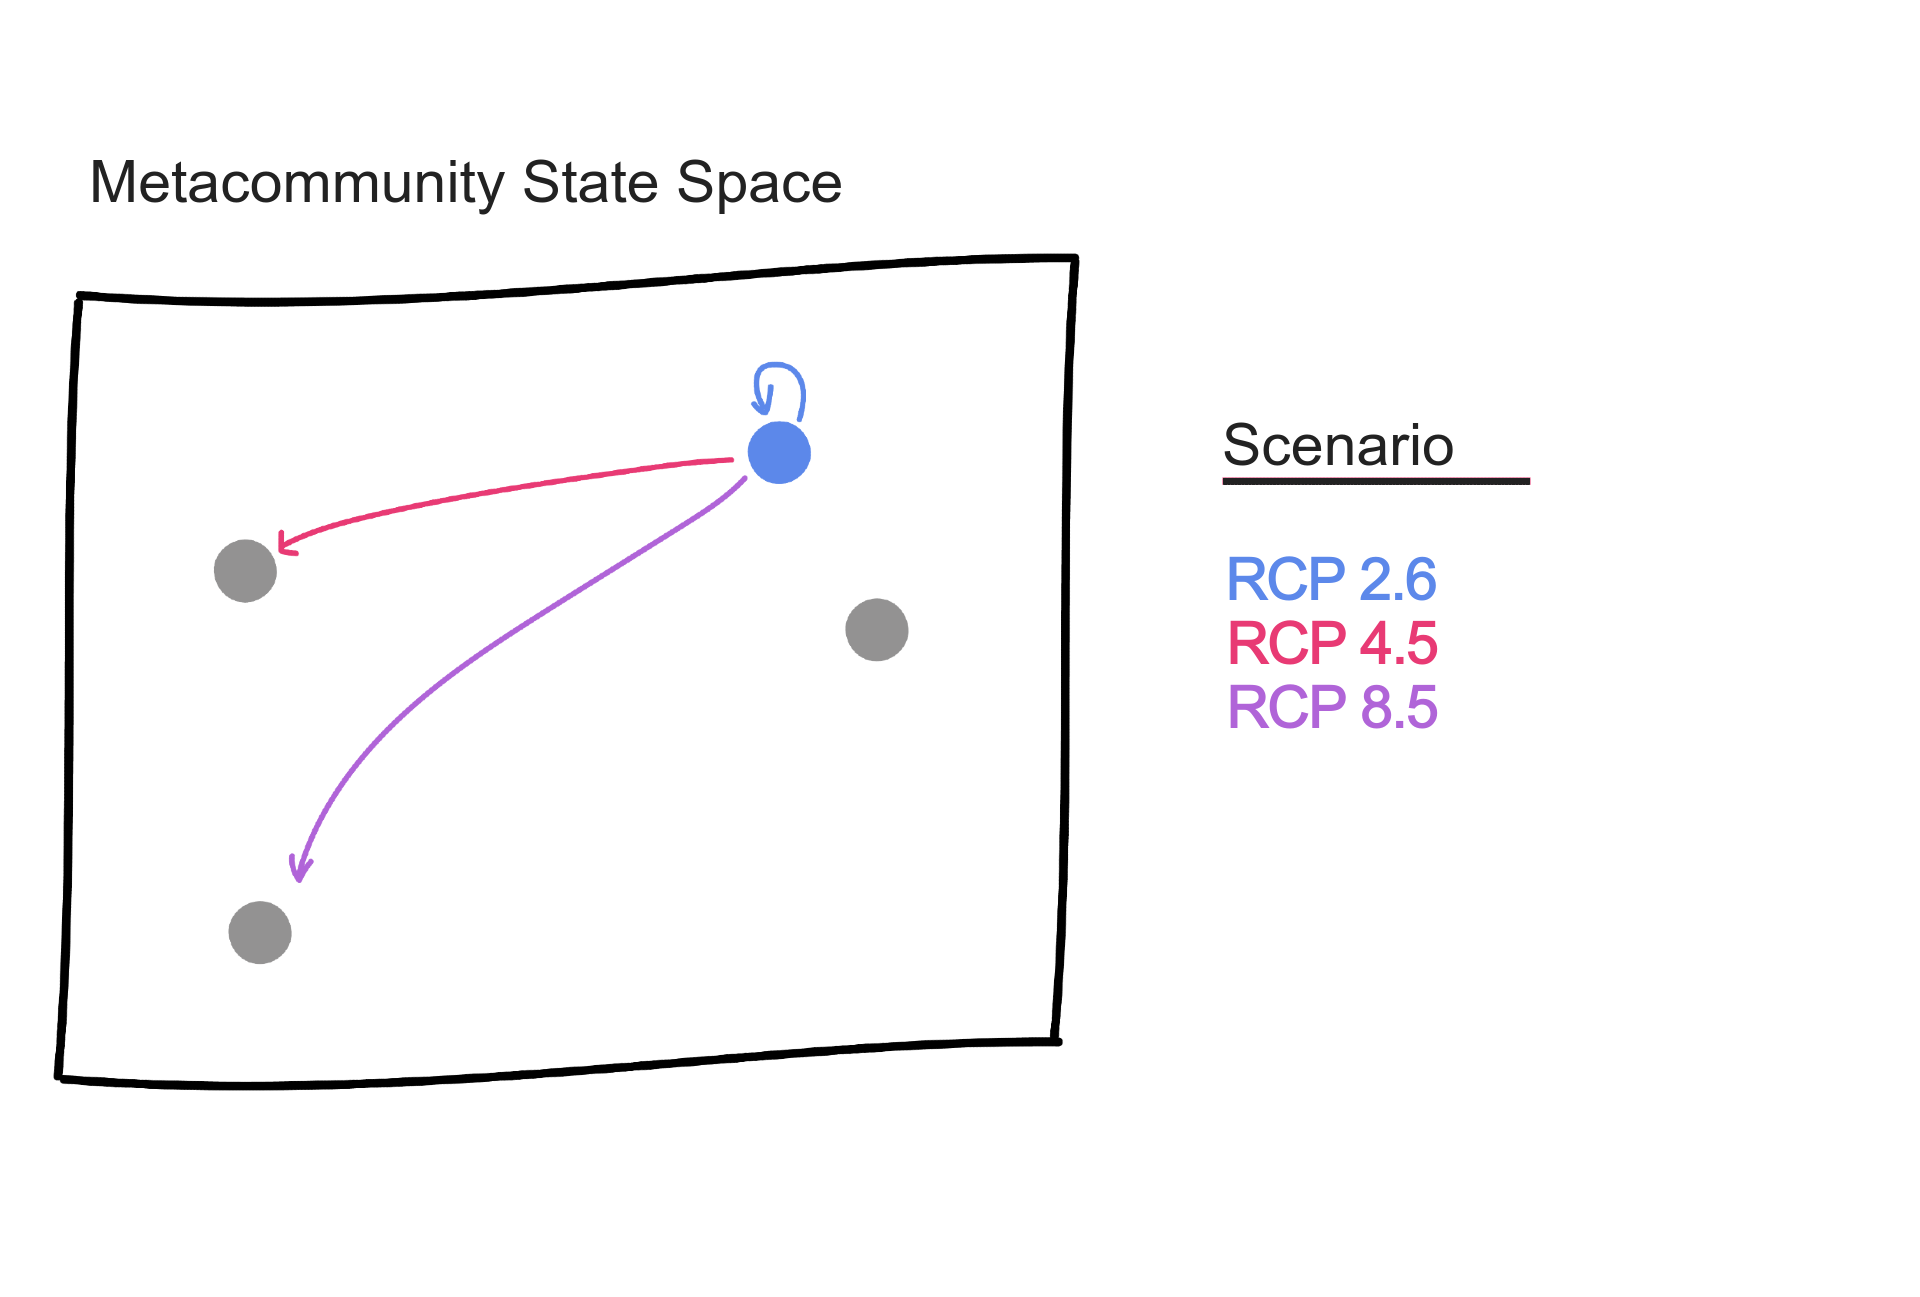
\includegraphics{/home/michael/prospectus/figures/different_scenarios.png}
\caption{this is a caption}
\end{figure}



% ________________________________________________________________________
%
%       CHAPTER 4
%
%           dissertation outline
%
% ________________________________________________________________________
\clearpage
\hypertarget{dissertation-outline}{%
\section{Dissertation Outline}\label{dissertation-outline}}

Here, we outline the structure of the five planned dissertation chapters.

\subsection{Chapter One}

An Introduction and Review Chapter, looks a lot like this document. 


\subsection{Chapter Two}

A Chapter about the Model, detailing the software and potentially applying it to reasonable data sets.
This chapter would be aimed at Methods in EcoEvo probably.

\subsection{Chapter Three}

Using the model as a virtual laboratory \citep{rollsback_agent_2005} to determine at what spatial scales do community assembly processes go from neutral to niche-based? We know that niche/neutrality are not opposing forces but instead shift along a continium (cite).


\begin{figure}[H]
\centering
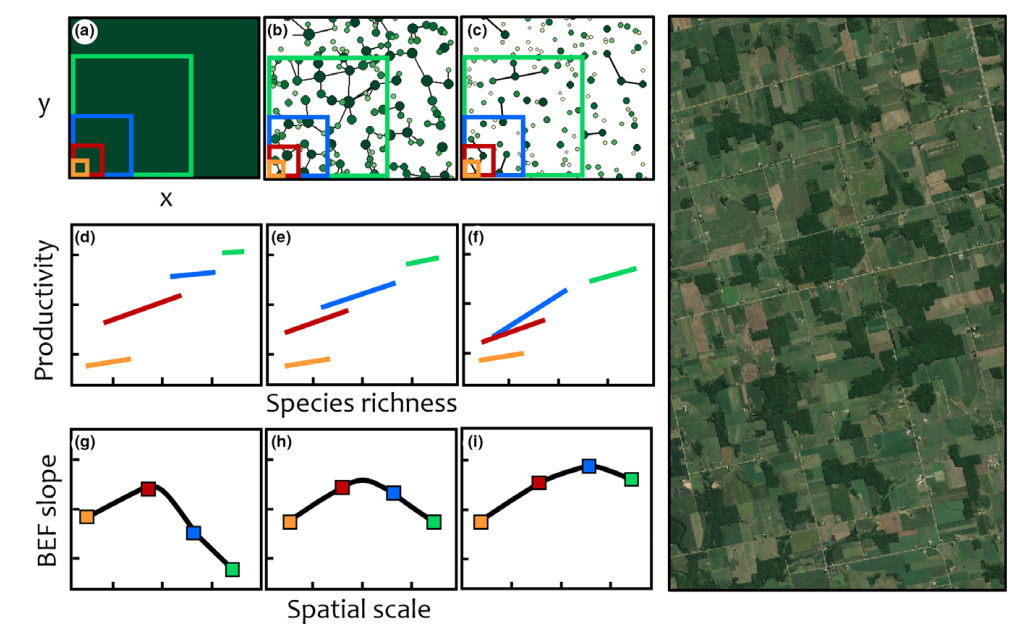
\includegraphics{/home/michael/prospectus/figures/gonzalez_ef_es.png}
\caption{this is a caption}
\end{figure}

\subsection{Chapter Four}
\subsection{Chapter Five}






% ________________________________________________________________________
%
%       REFERENCES
%
%
% ________________________________________________________________________
\clearpage
{
\footnotesize
\bibliography{refs}
}
There is still a reliance on summary statistics, but if summary
statistics are not differentiable even when the  generative process is
different, that is in itself is interesting, and, in general, simulation
models are excellent testing grounds for the biases of summary
statistics (see Jost's D vs Fst etc).

In the "virtual laboratory" case, the parameter values often are meant
to encapsulate the the entire spectrum of possible values, are based in
what the researcher (or reviewers) find interesting. In the second case,
parameter inference is vital in producing useful predictions.

\end{document}
